\chapter{基本的概念の解説}
本章では,本論文を理解する上で必要となる基本概念についての説明を行う.VCを理解するため材料として
エルミート行列の性質やべき乗法について説明する. \cite{strang} また,無線通信の理解に関してディジタル変復調,
同期検波等について説明を行う.

\section{数学的基礎知識}
VCを理解するための事前準備として数学的基礎知識の説明を行う.本章では行列の要素が複素数である
複素行列を扱っている.

\subsection{随伴行列(共役転置行列)}
ある複素行列$\bm{A}$において,全要素で共役をとった上でその行列を転置させたものを$\bm{A}$の随伴行列(共役転置行列)
といい,$\bm{A^H}$と表す.

(例)\quad
$
  \bm{A} = \left[
    \begin{array}{cc}
      1-i & 2-6i \\
      5+i & 3 \\
      0 & 1+9i
    \end{array}
  \right]
$とすると,
\vspace{1mm}
\begin{equation}
    \bm{A^H} = \left[
        \begin{array}{cc}
            1-i & 2-6i \\
            5+i & 3 \\
            0 & 1+9i
        \end{array}
    \right]^H 
    = \left[
        \begin{array}{ccc}
            1+i & 5-i & 0 \\
            2+6i & 3 & 1-9i \\
        \end{array}
    \right] \nonumber
\end{equation}

\subsection{複素ベクトルの内積}
要素数の等しい複素ベクトル$X,Y$の内積を,以下で定義する.
\begin{equation}
    (\bm{X},\bm{Y}) = \bm{X^HY}
\end{equation}

\subsection{任意ベクトルの表記}
M次元空間内の任意の列ベクトルを$\bm{x}$,M個の直交した固有ベクトルを$\bm{u_1},\bm{u_2},\ldots,\bm{u_M}$
とすると,$\bm{x}$はM個の固有ベクトル及び定数$c_i(i=0,1,\ldots)$を用いて,以下のように表すこと
ができる.
\begin{equation}
    \bm{x} = \sum_{i=1}^M c_i\bm{u_i}
\end{equation}

\section{エルミート行列}
ある複素行列$\bm{A}$において,$\bm{A}$の随伴行列$\bm{A^H}$が$\bm{A}$と等しいとき,$\bm{A}$を
エルミート行列と呼ぶ.

(例) \quad
$
  \bm{A} = \left[
    \begin{array}{cc}
      1 & 3-4i \\
      3+4i & 2
    \end{array}
  \right]
$とすると,
\vspace{1mm}
\begin{equation}
    \bm{A^H} = \left[
        \begin{array}{cc}
            1 & 3-4i \\
            3+4i & 2
        \end{array}
    \right]
    = \bm{A} \nonumber
\end{equation}
であり,$\bm{A^H}=\bm{A}$となることから$\bm{A}$はエルミート行列であると言える.

エルミート行列の主な性質として以下の4つが挙げられる.

\vspace{5mm}
\noindent\textbf{(性質1) \quad 任意複素ベクトルとの関係} \\
$\bm{A}$がエルミート行列であれば,任意の列ベクトル$\bm{x}$に対して,$\bm{x^HAx}$は実数になる.\\
\vspace{3mm}
(証明)

任意複素ベクトル
$
    \bm{x} = \left[
        \begin{array}{c}
            u \\
            v
        \end{array}
    \right]
$
,エルミート行列
$
    \bm{A} = \left[
        \begin{array}{cc}
            a & b \\
            b^* & c
        \end{array}
    \right]
$
とすると,
\begin{eqnarray}
    \bm{x^HAx} &=& 
    \left[
        \begin{array}{cc}
            u^* & v^*
        \end{array}
    \right]
    \left[
        \begin{array}{cc}
            a & b \\
            b^* & c
        \end{array}
    \right]
    \left[
        \begin{array}{c}
            u \\
            v
        \end{array}
    \right] \nonumber \\
    &=& auu^* + cvv^* + b^*uv^* + bu^*v \nonumber \\
    &=& a|u|^2+c|v|^2+b^*uv^*+bu^*v
\end{eqnarray}

\noindent(2.3)式の右辺第1項,第2項はともに実数である.第3項,第4項は互いに複素共役となっており,これらの
和は実数部分の2倍になる.よって,$\bm{x^HAx}$は実数であると言える.

\vspace{5mm}
\noindent\textbf{(性質2) \quad 全固有値が実数} \\
エルミート行列の固有値はすべて実数である. \\
\vspace{3mm}
(証明) \\
エルミート行列$\bm{A}$の固有値を$\bm{\lambda}$,その$\bm{\lambda}$に対応する$\bm{0}$でない
固有ベクトルを$\bm{x}$とする.行列とその行列の固有値・固有ベクトルとの関係より,
\begin{equation}
    \bm{Ax} = \lambda\bm{x}
\end{equation}
(2.4)式の両辺に$\bm{x^H}$をかけると,
\begin{equation}
    \bm{x^HAx} = \lambda\bm{x^Hx}
\end{equation}
(2.5)式の左辺は(性質1)により実数である.加えて,$\bm{x}\neq\bm{0}$より,$\bm{x^Hx}=||x||^2$
は正の実数である.したがって,$\lambda$は実数でなければならない.

\vspace{5mm}
\noindent\textbf{(性質3) \quad 固有ベクトルの直交性} \\
エルミート行列の固有ベクトルは,他のあらゆる固有値の固有ベクトルと直交している. \\
\vspace{3mm}
(証明) \\
ある$2\times2$以上の大きさを持ったエルミート行列$\bm{A}$の2つの異なる$\bm{0}$でない固有ベクトルを
$\bm{x}$,$\bm{y}$とし,$\bm{x}$,$\bm{y}$に対応する固有値を$\lambda,\mu(\lambda\neq\mu)$と
する.行列とその行列の固有値・固有ベクトルとの関係((2.4)式)より,
\begin{eqnarray}
    \bm{Ax} &=& \lambda\bm{x} \\
    \bm{Ay} &=& \mu\bm{y}
\end{eqnarray}
(2.6)式を共役転置すると,
\begin{equation}
    \bm{x^HA^H} = \lambda\bm{x^H} \hspace{10mm} (\because\lambda は実数より,\lambda=\lambda^*)
\end{equation}
$\bm{A}$はエルミート行列であることから$\bm{A=A^H}$.これを(2.8)式に代入して,
\begin{equation}
    \bm{x^HA} = \lambda\bm{x^H}
\end{equation}
(2.9)式の両辺に右から$\bm{y}$をかけると,
\begin{equation}
    \bm{x^HAy} = \lambda\bm{x^Hy}
\end{equation}
一方,(2.7)式の両辺に左から$\bm{x^H}$をかけると,
\begin{equation}
    \bm{x^HAy} = \mu\bm{x^Hy}
\end{equation}
これら(2.10)式,(2.11)式より,
\begin{equation}
    \lambda\bm{x^Hy} = \mu\bm{x^Hy}
\end{equation}
$\lambda\neq\mu$であることから,$\bm{x^Hy}=\bm{0}$でなければならない.$\bm{x^Hy}$は
複素列ベクトル$\bm{x},\bm{y}$の内積を表しており((2.1)式),それが$\bm{0}$であるということは
$\bm{x}$と$\bm{y}$は直交関係にある.

\vspace{5mm}
\noindent\textbf{(性質4) \quad スペクトル定理} \\
エルミート行列$\bm{A}$はその固有ベクトル群行列$\bm{U}$,固有値対角行列$\bm{D}$を用いて,
次のように分解できる. \\
\begin{eqnarray}
    \bm{A} &=& \bm{UDU^H} = c_1\lambda_1\bm{u_1u_1^H}+c_2\lambda_2\bm{u_2u_2^H}+\ldots+c_n\lambda_n\bm{u_nu_n^H} \nonumber \\
    &=& \sum_i c_i\lambda_i\bm{u_iu_i^H}
\end{eqnarray}
\vspace{3mm}
(証明) \\
あるエルミート行列$\bm{A}$の固有値・固有ベクトルをそれぞれ$\lambda_i,\bm{u_i}$とする.
$\bm{u_i}$は正規直交基底であるから,任意ベクトル$\bm{x}$は(2.2)式のように分解される.
$\bm{x}$に左から$\bm{A}$をかけると,
\begin{equation}
    \bm{Ax} = \sum_i c_i\bm{Au_i} = \sum_i c_i\bm{\lambda u_i}
\end{equation}
が得られる.一方,(2.13)式の右辺に$\bm{x}$をかけると,
\begin{equation}
    \left[
        \sum_k \lambda_k\bm{u_ku_k^H}
    \right]\bm{x}
    = \left[
        \sum_k \lambda_k\bm{u_ku_k^H}
    \right]\sum_i c_i\bm{u_i}
    = \sum_{i,k} c_i\lambda_k\bm{u_ku_k^Hu_i}
    = \sum_i c_i\lambda_i\bm{u_i} \nonumber
\end{equation}
となり,これは(2.14)式と一致する.以上より,(2.13)式が成立することが証明された.

\section{べき乗法}
対角行列の固有値・固有ベクトルを求める方法の一つにべき乗法がある.$\bm{A}$をM次のエルミート行列
とし,その固有値を$\lambda_1,\lambda_2,\ldots,\lambda_M$とする.$\lambda_i$に対応する
固有ベクトルを$\bm{u_i}$とすると,(2.4)式より,
\begin{equation}
    \bm{Au_i} = \lambda_i\bm{u_i} \nonumber
\end{equation}
となる.以下では,$|\lambda_1|>|\lambda_2|>\cdots>|\lambda_M|$の関係があるとする.
任意ベクトル$\bm{x}$に左から$\bm{A}$をn回乗算したものを$\bm{x_n}$とする.$\bm{x}$に左から
$\bm{A}$を1回乗算すると,
\begin{eqnarray}
    \bm{x_1} &=& \bm{Ax_0} = \bm{A}\sum_{i=1}^M c_i\bm{u_i} \hspace{10mm}(\because(2.2)式) \nonumber \\
    &=& \sum_{i=1}^M c_i\bm{Au_i} = \sum_{i=1}^M c_i\lambda_i\bm{u_i}
\end{eqnarray}
である.(2.15)式に繰り返し左から$\bm{A}$を1回乗算すると,
\begin{eqnarray}
    \bm{x_2} &=& \bm{Ax_1} = \bm{A^2x_0} = \sum_{i=1}^M c_i\lambda_i^2\bm{u_i} \nonumber \\
    \bm{x_3} &=& \bm{Ax_2} = \bm{A^3x_0} = \sum_{i=1}^M c_i\lambda_i^3\bm{u_i} \nonumber \\
    \vdots \nonumber
\end{eqnarray}
となり,$\bm{x_n}$は下記のようになる.
\begin{eqnarray}
    \bm{x_n} &=& \sum_{i=1}^M c_i\lambda_i^n\bm{u_i} \nonumber \\
    &=& \lambda_1^n
    \left(
        c_1+\bm{u_1}+\sum_{i=2}^M c_i
        \left(
            \frac{\lambda_i}{\lambda_1}
        \right)^n
        \bm{u_i}
    \right)
\end{eqnarray}
(2.16)式において,nが十分に大きい($\bm{A}$の乗算を十分繰り返す)場合,
\begin{equation}
    \left|\frac{\lambda_i}{\lambda_1}^n\right| << 1 \hspace{10mm} (i=2,3,\ldots,M)
\end{equation}
であるから,(2.16)式,(2.17)式より,
\begin{equation}
    \bm{x_n} = \lambda_1^nc_1\bm{u_1}
\end{equation}
が導かれる.(2.18)式は,任意ベクトル$\bm{x}$に繰り返し$\bm{A}$を乗算することで$\bm{x}$が
$\bm{A}$の第1(最大)固有ベクトル$\bm{u_1}$の定数倍に近づいていくことを意味している.
$\bm{x_n}$と$\bm{u_1}$は,大きさは違うが方向は同じであるため,$\bm{x_n}$を正規化することで
$\bm{u_1}$が得られる.正規化とはベクトルの各成分をベクトルの長さ(ノルム)で割ることにより,
ベクトルを単位ベクトルにすることである.

nを十分大きく取り$\bm{u_1}$を引き込んだ後,$\bm{u_1}$に$\bm{A}$を乗算することで$\bm{u_1}$に
対応する固有値$\lambda_1$は得られる.つまり,$\bm{u_1}$に$\bm{A}$を乗算した結果を$\bm{u_1^{\prime}}$
とすると,$\bm{u_1^{\prime}}$は$\bm{u_1}$の定数倍となり,この定数が固有値$\lambda_1$である.

エルミート行列$\bm{A}$はスペクトル定理により,(2.13)式のように分解できる.(2.13)式と一致する.以上より,
\begin{equation}
    \bm{A} - \lambda_1\bm{u_1}\bm{u_1^H} = \lambda_2\bm{u_2}\bm{u_2^H} + \cdots + \lambda_n\bm{u_n}\bm{u_n^H}
\end{equation}
であるから,(2.19)式の左辺$\bm{A} - \lambda_1\bm{u_1}\bm{u_1^H}$($\bm{A_2}$とする)の
第1固有値・固有ベクトルは,$\bm{A}$の第2固有値・固有ベクトルに当たる.すなわち,$\bm{A}$から
第1固有値・固有ベクトルを導出した手順を$\bm{A_2}$に適用することで,$\bm{A}$の第2固有値・
固有ベクトルが得られる.第2以降の固有値・固有ベクトルも,第2固有値・固有ベクトルと同様の手順で得られる.

\section{最適化問題の解法}
最適化問題は,与えられた制約条件の下で,目的関数と呼ばれる望ましさの尺度を表す関数が最小または最大となるような
決定変数の値を見つける,という数学モデルとして定式化できる. \cite{ibaragi}
最適化問題は,まず目的関数が線形関数か非線形関数かで大きく二つに分けることができる.そこからさらに,
制約条件の等号,不等号や決定変数が連続か非連続かによって細分化される.
一般に非線形関数の最適化の方が線形関数の最適化よりも困難とされる.

\subsection{KKT条件(Karush-Kuhn-Tucker condition)}
次のような不等式制約を持つ最適化問題を考える.

\begin{equation}
    \left\{
        \begin{array}{cc}
            目的関数:f(x) \to 最小 & \\
            制約条件:c_i(x) \leq 0 & (i=1,2,\ldots,m)
        \end{array}
    \right.
\end{equation}

ただし,変数$x$はn次元実ベクトルであり,目的関数$f:R^n \to R$および制約関数
$c_i:R^n \to R(i=1,\ldots,m)$はともに2回連続微分可能と仮定する.
まず,点$x$を(2.34)の実行可能解としたとき,$c_i(x)=0$が成り立つ制約条件を点$x$における有効制約
とよび,その集合を

\begin{equation}
    I(x) = {i| \quad c_i(x)=0 \hspace{10mm} (i=1,2,\ldots,m)} \nonumber
\end{equation}

で表す.さらに,有効制約の勾配ベクトル$\nabla c_i(x)(i \in I(x))$が1次独立であるような点$x$を
正則点という.

次の定理に示される条件は,非線形最適化問題の最適解を特徴づける重要な条件であり,KKT
(\emph{KKT: Karush Kuhn Tucker})条件と呼ばれる.\cite{ibaragi}

点$x^*$が(2.34)の局所的最適解かつ正則点ならば,

\begin{equation}
    \left\{
        \begin{array}{cccc}
            \nabla f(x^*)+\sum_{i=1}^m u_i^*\nabla c_i(x^*)=0 & & & \\
            c_i(x^*)\leq0, & u_i^*\geq0, & u_i^*c_i(x^*)=0 & (i=1,2,\ldots,m)
        \end{array}
    \right.
\end{equation}
を満たすベクトル$u^*=(u_1^*,u_2^*,\ldots,u_m^*)$が存在する.
ベクトル$u^*$をラグランジュ乗数と呼ぶ.

\subsection{ラグランジュの未定乗数法}
変数$\bm{x}$の関数$f(\bm{x})$の最大値,最小値は,等式制約$g(\bm{x})=0$が存在する場合,
ラグランジュ乗数$\lambda$を導入した

\begin{equation}
    F = f(\bm{x}) - \lambda g(\bm{x})
\end{equation}

を考え,これを$\bm{x}$で微分して$\bm{0}$と置く.

\begin{equation}
    \nabla_{\bm{x}}f - \lambda\nabla_{\bm{x}}g = \bm{0}
\end{equation}

これと等式制約$g(\bm{x})=0$を連立させて解けば,$\bm{x}$と$\lambda$を定めることができる.
この解法をラグランジュの未定乗数法と呼ぶ. \cite{kanatani}
ラグランジュの未定乗数法は線形最適化問題の解法として一般的である.
また,制約条件に不等式制約が存在する場合を考えるとき,ラグランジュの未定乗数法を
拡張した,2次計画法と呼ばれる解法が用いられる.
2次計画法を用いることでKKT条件の最適化問題を解くことができる.

\section{ディジタル変復調}
無線通信では,情報源のベースバンド信号(変調信号)を搬送波を用い,搬送波周波数帯の
信号に変換することが必要である.ベースバンド信号を伝送に適した形に変換することを変調と
呼び,逆の操作を復調と呼ぶ.これらの処理を合わせて変復調と呼び,その中でも情報源がディ
ジタルデータのものをディジタル変復調と呼ぶ\cite{takahata}.変調では,搬送波の振幅や周波数,位相な
どの性質を変化させることにより,信号を変換する.

\subsection{ディジタル変調}
\subsubsection{QPSK(Quadrature Phase Shift Keying)}
位相を用いて変調するものを位相偏移変調(PSK:Phase Shift Keying)と呼ぶ.
PSKでは,2進ディジタル信号を$n$ビットずつまとめ,これに対し$M=2^n$の位相を割り当てることで
搬送波に情報を持たせる.これを一般に$M$相PSKと呼び,
次の式で表される\cite{saitou}\cite{okumura}.
\begin{eqnarray}
\left\{
\begin{array}{ll}
\displaystyle s(t)=\mbox{Re}\left[Ae^{j(\omega_c t+\phi_m)}\right]&(-T/2 \leq t \leq T/2) \\[2mm]
\displaystyle \phi_m = \frac{2\pi}{M}(m-1) & (m=1,2, \cdots ,M)
\end{array}
\right.
\label{no2-6}
\end{eqnarray}
$M$相PSKの中でも$M$=4の場合を4位相偏移変調(QPSK:Quadrature Phase Shift Keying)と呼び,
$\phi_m=\pi/4,  3\pi/4,  5\pi/4,  7\pi/4$ が用いられる \cite{okumura}.
QPSK信号$S_{{\rm QPSK}}(t)$は,
\begin{eqnarray}
S_{{\rm QPSK}}(t)&=&\mbox{Re}\left[Ae^{j(\omega_c t +\phi_m)} \right] \nonumber \\
&=&\mbox{Re}\left[\left\{A\cos\phi_m+jA\sin\phi_m\right\}e^{j\omega_c t}\right] \nonumber \\[1mm]
&=&\mbox{Re}\left[\left\{Ad_1(t)+jAd_2(t) \right\}e^{j\omega_c t}\right] \nonumber \\[1mm]
&=&Ad_1(t)\cos\omega_ct-Ad_2(t)\sin\omega_ct
\label{eqqpsk}
\end{eqnarray}
と表される.ここで,
\begin{eqnarray}
\left\{
\begin{array}{ll}
\displaystyle \phi_m = \frac{2\pi}{4}(m-1)+\frac{\pi}{4} \hspace{2mm}(m=1,\cdots ,4) \\[2mm]
\displaystyle d_1 = \cos \phi_m \hspace{16mm}(=\pm1) \\[1mm]
\displaystyle d_2 = \sin \phi_m \hspace{16.5mm}(=\pm1)
\end{array}
\right.
\label{ff}
\end{eqnarray}
である.つまり,QPSKではこの4つの位相を2ビットの系列00,01,10,11に対応させて伝送する.
QPSK変調の信号点配置および,変調器の回路図を図\ref{fig:qpskIQ},図\ref{fig:qpskmod}に示す.
信号点配置はグレイコードが用いられ,隣接する信号点のハミング距離が1となるように設定されている.
%----------------------------画像をいれた----------------------------
\begin{figure}[t]
  \begin{center}
    \includegraphics[scale = 0.25]{./chapter2/figure/qpskiq.eps}
    \caption{QPSK変調の信号点配置の例}
    \label{fig:qpskIQ}
  \end{center}
\end{figure}
\begin{figure}[t]
  \begin{center}
    \includegraphics[scale = 0.25]{./chapter2/figure/qpskshift.eps}
    \caption{QPSK変調の回路図}
    \label{fig:qpskmod}
  \end{center}
\end{figure}

\subsection{同期検波}
変調された信号(被変調信号)から元の信号を得ることを復調という.復調方式として図 \ref{fig:qpskcoh} に示すような同期検波を考える.同期検波とは,変調側と同位相の搬送波を用い,受信信号との積をとることにより,元の変調信号を得る方法である\cite{takahata}.QPSK信号$S_{{\rm QPSK}}(t)$に$\cos\omega_c t$,$-\sin\omega_c t$をかけたものをそれぞれ$m_1(t), m_2(t)$とすると,
\begin{eqnarray}
m_1(t)&=&Ad_1(t)\cos^2\omega_ct+Ad_2(t)\sin\omega_ct\cos\omega_ct \nonumber \\
&=&\frac{1}{2}Ad_1(t)+\frac{1}{2}Ad_1(t)\cos2\omega_ct+\frac{1}{2}Ad_2(t)\sin2\omega_ct \\
m_2(t)&=&-Ad_1(t)\sin\omega_ct\cos\omega_ct+Ad_2(t)\sin^2\omega_ct \nonumber \\
&=&\frac{1}{2}Ad_2(t)-\frac{1}{2}Ad_2(t)\cos2\omega_ct-\frac{1}{2}Ad_1(t)\sin2\omega_ct
\end{eqnarray}
となる.ここで,$m_1(t)$,$m_2(t)$をローパスフィルタ(LPF:Low-Pass Filter)に通すことにより高周波成分を除いたものを$\hat{m}_1(t)$,$\hat{m}_2(t)$とすると,
\begin{eqnarray}
\hat{m}_1(t)&=&\frac{1}{2}Ad_1(t)\\
\hat{m}_2(t)&=&\frac{1}{2}Ad_2(t)
\end{eqnarray}
となる.$\hat{m}_1(t)$,$\hat{m}_2(t)$を並直列変換(parallel / serial conversion)することで,元の信号が復元される.
%------------------------------仮画像------------------------------
\begin{figure}[t]
  \begin{center}
    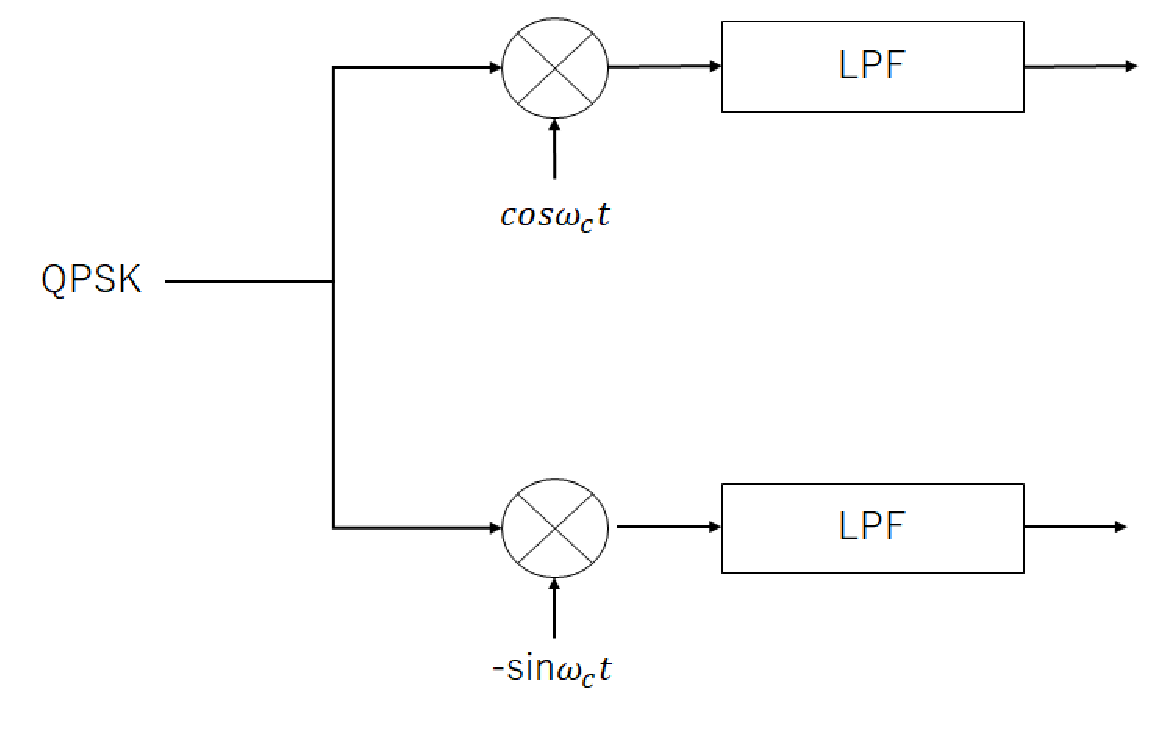
\includegraphics[scale = 0.25]{./chapter2/figure/douki.eps}
    \caption{QPSK変調の同期検波回路}
    \label{fig:qpskcoh}
  \end{center}
\end{figure}
%------------------------------------------------------------------

\subsection{信号の等価低域表現}
対象システムの特性をコンピュータシミュレーションのような離散時間処理によって評価する場合,サンプリング定理を満足するなるべく小さなサンプリング周波数を用い,演算量を削減することが望ましい.そこで本研究では,信号を複素ベースバンドで表現し,等価低域表現によるシミュレーションを行っている.

ここで,ベースバンド信号の帯域幅が$B[{\rm Hz}]$のQPSK変調信号を考える.搬送波の周波数が$f_c[{\rm Hz}]$である場合,信号の最高周波数が$f_c+B[{\rm Hz}]$となるため,標本化定理により,この信号は$2(f_c+B)[{\rm Hz}]$以上で標本化する必要がある.一方,式(\ref{eqqpsk})より,QPSK変調信号の複素数表現は,$\{Ad_1(t)+jAd_2(t)\}e^{j2\pi f_ct}$となる.複素数表現では,$f_c=0$として,複素ベースバンド信号で表すことができ,
\begin{eqnarray}
b(t)=Ad_1(t)+jAd_2(t)
\end{eqnarray}
となる.標本化定理から,$2B[{\rm Hz}]$以上でサンプリングすれば復調できるため,実信号表現の場合と比べてサンプリング周波数を低くすることができ,サンプル点数を減らすことができる.この表現方法を等価低域表現と呼ぶ\cite{takahata}.
%------------------------------------------------------------------------

\section{フェージング伝搬路の影響}
開空間を伝送媒体として用いる無線通信では,気象条件や地理的条件によってその伝搬路特性が変化する.
また,通信中に場所の移動が伴う場合は伝搬路特性の変動が更に厳しいものとなる.
この現象はフェージングと呼ばれ,送信信号に振幅変動や位相変動を発生させる.
その結果,受信信号の品質は顕著な影響を受ける \cite{saitou}.

\subsection{マルチパスフェージングの発生原理}
送信された電波は大気屈折率の変化や大地,山,建物,あるいは車等によって反射,回折,散乱する.
材質や入射角により,ある電波は大きな減衰を受け,ある電波はほとんど減衰せずに経路が変えられるなど
して,マルチパス伝搬路が形成される(図 \ref{fig:multipath}).

受信点では多数の波が干渉し,定在波が生じる.この中を移動すると到来する多数の波の干渉により
激しい振幅時間変動,位相時間変動が生じる.
この現象をフェージングと呼ぶ\cite{okumura}.
簡単な例として,複素搬送波$e^{j2\pi f_ct}$が伝送され,図 \ref{fig:coming_waves}のように,マルチパス伝搬路において複数の散乱波が受信される場合を考える.$n$番目のパスを通過した信号の振幅を$a_n(t)$,位相を$\theta_n(t)$とすれば,そのときの受信信号$r_n(t)$は,
\begin{eqnarray}
r_n(t)&=&{\rm Re}\left[a_n(t)e^{j2\pi f_c t+j\theta_n(t)}\right]\nonumber \\
&=&{\rm Re}\left[z_n(t)e^{j2\pi f_c t}\right]
\end{eqnarray}
となる.ここで$z_n(t)\equiv a_n(t)e^{j\theta_n(t)}$とし,$r_n(t)$の複素包絡線を表す.また,$a_n(t)$は複素包絡線$z_n(t)$の振幅変化,$\theta_n(t)$は複素包絡線$z_n(t)$の位相変化をそれぞれ表す.したがって,受信信号$r(t)$は,
\begin{eqnarray}
r(t)=\sum_{n=1}^{N}z_n(t)e^{j\pi f_ct}
\end{eqnarray}
となる.ここで,受信点や周囲の環境が静止している場合には,$a_n(t)$,$\theta_n(t)$はほとんど変化せず,準静的フェージングモデルを与える.一方,受信点が速度$v$で移動すると,到来角度$\phi_n$に応じて,$v\cos(\phi_n)/\lambda$のドップラー周波数変動を受け,動的フェージングモデルとなる.このとき,初期位相を$\varphi_n$とすると,$\theta_n(t)$は,
\begin{eqnarray}
\theta_n(t)=2\pi\frac{vt\cos\phi_n}{\lambda}+\varphi_n
\end{eqnarray}
となる.ここで,$v/\lambda=f_D$は最大ドップラー周波数といわれるものであり,物理的には移動局の進行方向($\phi_n=0$)からの到来波周波数が$f_D[{\rm Hz}]$だけ高くなるのに対して,後方($\phi_n=\pi$)からの到来波は$f_D[{\rm Hz}]$だけ低くなることを表す.
\begin{figure}[t]
  \begin{center}
    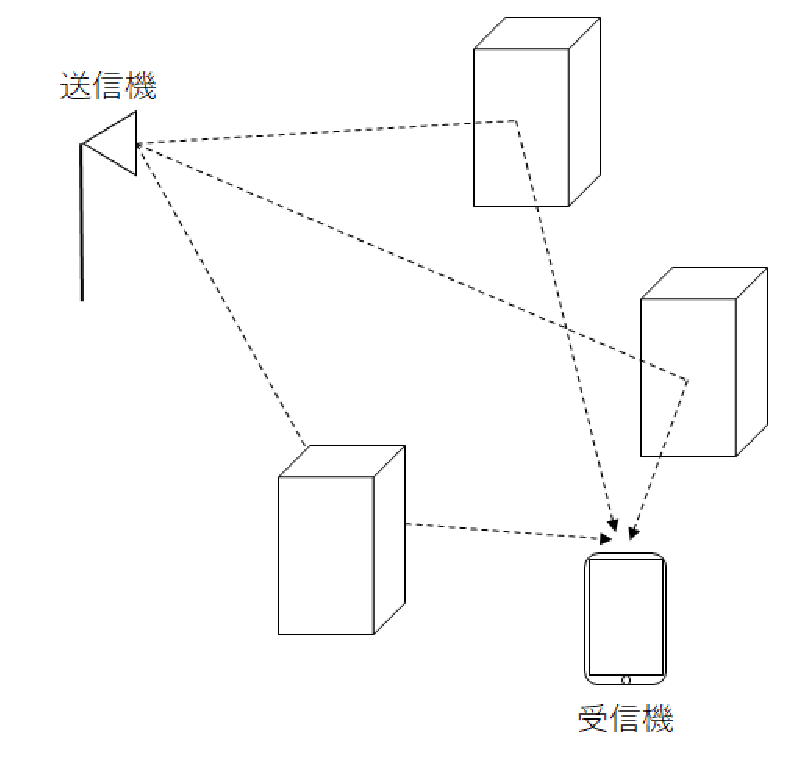
\includegraphics[scale = 0.25]{./chapter2/figure/multipaths.eps}
    \caption{マルチパス伝搬路モデル}
    \label{fig:multipath}
  \end{center}
\end{figure}

\begin{figure}[htbp]
	\begin{center}
		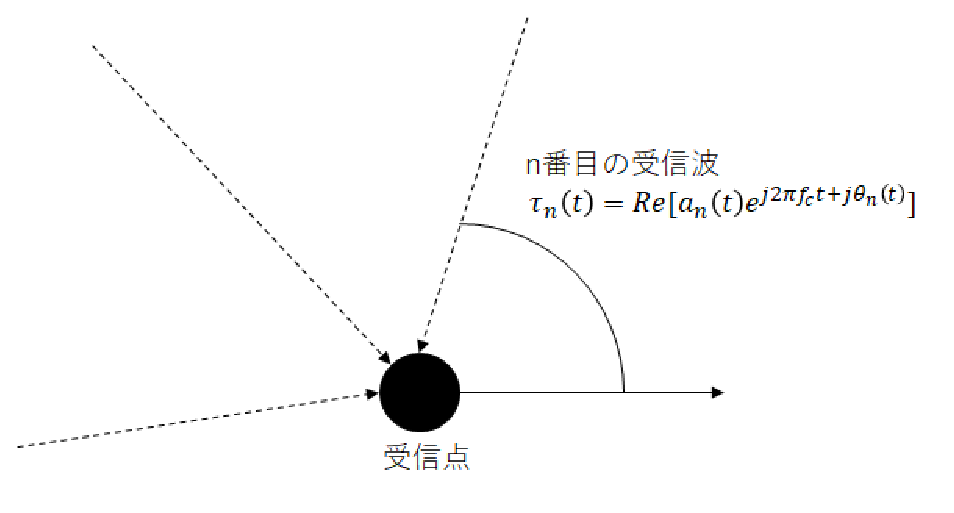
\includegraphics[scale=0.15]{./chapter2/figure/jushin.eps}
		\caption{マルチパス伝搬路の受信モデル}
		\label{fig:coming_waves}
	\end{center}
\end{figure}
%--------------------------------------------------------------------------------

\subsection{レイリーフェージング}
到来する素波数を$N$とする.このとき,受信信号$r(t)$の複素包絡線$z(t)$は,
\begin{eqnarray}
z(t)&=&\sum_{n=1}^{N}z_{n}(t) \nonumber \\
%&=&\sum_{n=1}^{N} a_{n}(t)e^{j\theta_{n}(t)} \nonumber \\
&=&\sum_{n=1}^{N}x_n(t)+j\sum_{n=1}^{N}y_n(t) \nonumber \\
&=& x(t)+j y(t)
\end{eqnarray}
となる.ここで,$x(t)$と$y(t)$はそれぞれ$z(t)$の同相成分,直交成分を表す.$x(t)$と$y(t)$は各波の強さが同程度である正弦波の和とすると,中心極限定理より$x(t)$,$y(t)$は平均値が0で等しい分散を持つ互いに独立な定常ガウス(Gauss)過程となる.$x=x(t)$,$y=y(t)$の結合確率密度関数$p(x,y)$は,
\begin{eqnarray}
p(x,y)=\frac{1}{2\pi \sigma^2}{\rm exp}\left(-\frac{x^2+y^2}{2\sigma^2}\right)
\end{eqnarray}
と表せる.ここで,$\sigma^2$は$r(t)$の平均受信電力である.包絡線振幅を$r$,位相を$\theta$とすると,
\begin{eqnarray}
\begin{cases}
r=\sqrt{x^2+y^2}& \\[4pt]
\theta=\tan^{-1}\left(\displaystyle \frac{y}{x}\right)&
\end{cases}
\end{eqnarray}
の関係がある.ここで,同相・直交成分の振幅が$(x, x+dx), (y, y+dy)$の領域に存在する確率は,デカルト座標から極座標に変換しても変わることはないため,次の式が成立する.
\begin{eqnarray}
\left\{
\begin{array}{ll}
p(x,y)dx\cdot dy & =p(r,\theta)dr\cdot d\theta  \\[12pt]
dx\cdot dy & =r\cdot dr\cdot d\theta
\end{array}
\right.
\end{eqnarray}
したがって,
\begin{eqnarray}
p(r,\theta)=\frac{r}{2\pi \sigma^2}{\rm exp}\left(-\frac{r^2}{2\sigma^2}\right)
\end{eqnarray}
となる.以上より,包絡線の確率密度関数$p(r)$と位相の確率密度関数$p(\theta)$は以下のように求められる.
\begin{eqnarray}
\left\{
\begin{array}{ll}
p(r)=\displaystyle \int_0^{2\pi}p(r,\theta)=\frac{r}{\sigma^2}{\rm exp}\left(-\frac{r^2}{2\sigma^2}\right)&(0\leq r \leq \infty)\\[12pt]
p(\theta)=\displaystyle \int_0^\infty p(r,\theta)dr=\frac{1}{2\pi} & (0\leq\theta\leq2\pi)
\end{array}
\right.
\end{eqnarray}
\begin{figure}[t]
	\begin{center}
		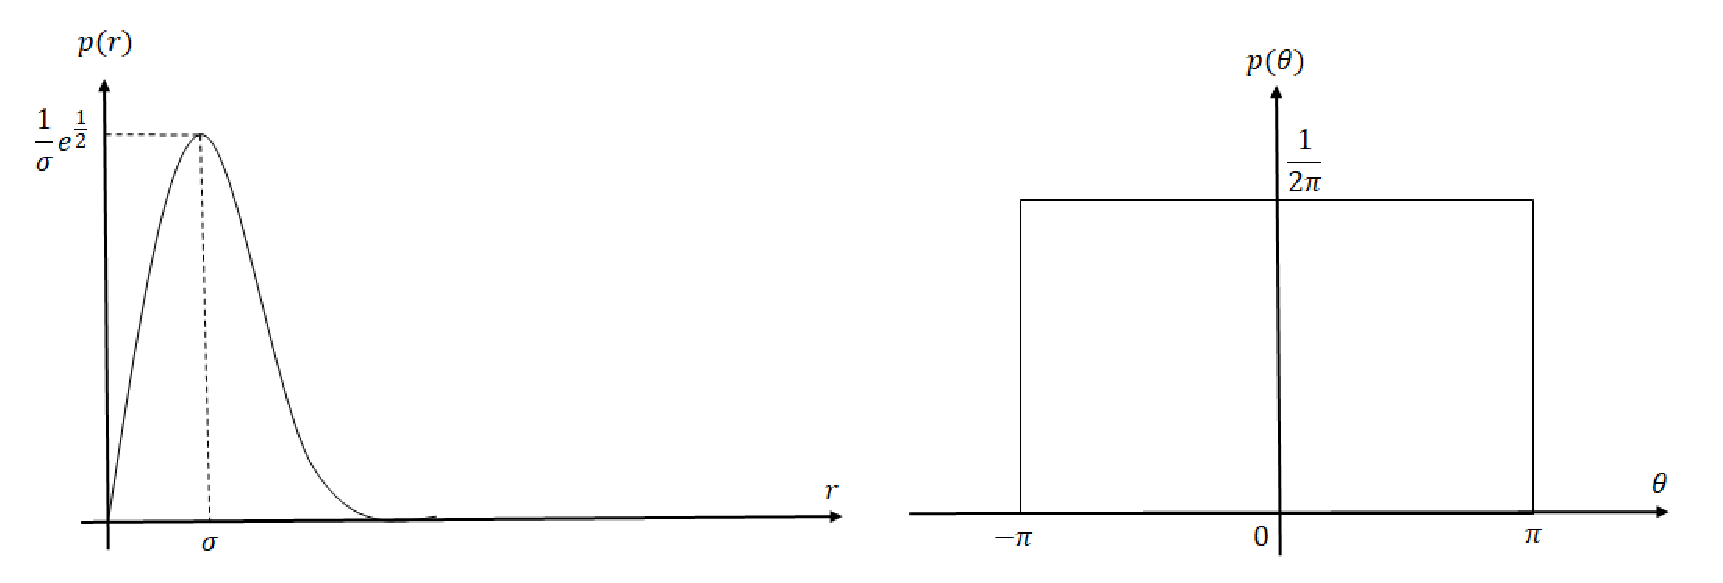
\includegraphics[scale=0.14]{./chapter2/figure/hourakusen.eps}
		\caption{包絡線と位相の確率密度関数}
		\label{figrayleigh}
	\end{center}
\end{figure}
$p(r)$,$p(\theta)$を図 \ref{figrayleigh}に示す.包絡線と位相の変動はそれぞれレイリー分布と一様分布に従うことがわかる.このようなフェージングをレイリーフェージングと呼ぶ\cite{saitou}\cite{okumura}.
%------------------------------------------------------------------------------